\renewcommand{\thesection}{S3}
\section{Design Basis: State of the Art, Requirements \& Specifications, and Benchmarking}

\subsection{State-of-the-Art Rovers in Planetary Exploration}

    \subsubsection{Zhurong: Active Suspension for Adaptability}
        Figure \ref{fig:Zhurong} shows China's Zhurong rover, which features an advanced active suspension system that independently adjusts each wheel's position and load \cite{CNSA_Zhurong}. This design improves performance on loose soils and steep inclines, such as those found in Mars' Utopia Planitia region.
        
        Its aluminum-silicon carbide composite wheels are lightweight yet strong, while its six-wheeled configuration reduces ground pressure \cite{Zhurong_Mission_Analysis_2021}. On Titan, where gravity is lower than Earth's, and the surface includes methane lakes and frozen ground, an active suspension system could enhance the ability to navigate these diverse terrains. Zhurong's approach highlights the importance of independent control for achieving stability and mobility.

        \renewcommand{\thefigure}{S1}
        \begin{figure}[ht]
            \centering
            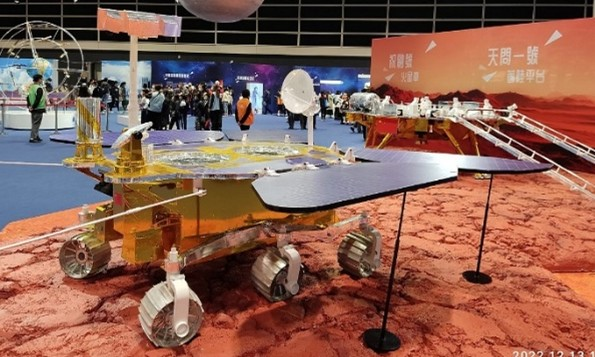
\includegraphics[height=6cm]{Figures/Zhurong.jpg}
            \caption{Full-scale mockup of Zhurong rover \cite{Wikipedia_Zhurong}. Image by AKAMGO yalms (CC BY-SA 4.0).}
            \label{fig:Zhurong} 
        \end{figure}
        \vspace{-20pt} % Adjust this value to reduce the space
        \FloatBarrier

    \subsubsection{VIPER: Navigating the Lunar South Pole}
        NASA's VIPER rover, presented in Figure \ref{fig:VIPER}, is tailored to operate in the extreme environment of the Moon's south pole \cite{NASA_Viper_Project}. It uses a four-wheel independent suspension system with active articulation, enabling precise manoeuvring such as "crab-walking" over steep slopes and loose regolith.
        
        VIPER's design incorporates lightweight composites and advanced thermal systems to withstand temperature extremes and abrasive lunar dust \cite{NASA_Viper_Rover}. With its cryogenic temperatures and potential for surface liquid hydrocarbons, Titan's environment would benefit from similar thermal management solutions. VIPER's mobility system also suggests how active articulation could address Titan's challenging topography.

        \renewcommand{\thefigure}{S2}
        \begin{figure}[ht]
            \centering
            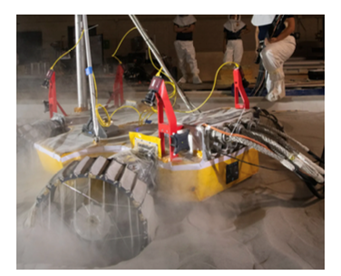
\includegraphics[height=6cm]{Figures/VIPER.png}
            \caption{The VIPER engineering team observe the rover prototype’s ability to navigate the fluffy lunar soil simulant in the SLOPE lab at NASA’s Glenn Research Center in Cleveland \cite{NASA_Viper_Prototype}.}
            \label{fig:VIPER} 
        \end{figure}
        \vspace{-20pt} % Adjust this value to reduce the space
        \FloatBarrier